\documentclass[10pt,epsf]{article}
\usepackage{geometry}[lmargin=0.5in,rmargin=0.5in]
\usepackage{amssymb,amsmath,amsthm,amsfonts,mathrsfs,color}
\usepackage{mathtools,commath}
\usepackage{epsfig}
\usepackage{latexsym}
\usepackage{verbatim}
\usepackage{setspace}
\usepackage{algorithm}
\usepackage[noend]{algorithmic}
\usepackage{algorithmicext}
\usepackage{ifthen}
\usepackage{graphicx}
\usepackage{grffile}
\usepackage{pgfplots}
\usepackage{longtable}
\usepackage{url}
\usepackage{hyperref}
\usepackage[utf8]{luainputenc}
\usepackage[bibencoding=utf8,backend=biber]{biblatex}
\addbibresource{cosc6342-hw2-michael-yantosca.bib}
\usepackage{chngcntr}
\counterwithin{figure}{subsection}
\usepackage{minted}
\usepackage{fancyhdr}
\pagestyle{fancy}
\lhead{{\footnotesize{COSC6342 HW 2}}}
\rhead{{\footnotesize{Michael Yantosca}}}

\newtheorem{fact}{Fact}
\newtheorem{theorem}{Theorem}
\newtheorem{lemma}{Lemma}
\newtheorem{claim}{Claim}
\newtheorem{remark}{Remark}
\newtheorem{definition}{Definition}
\newtheorem{corollary}{Corollary}
\newtheorem{proposition}{Proposition}
\newtheorem{example}{Example}
\newtheorem{observation}{Observation}
\newtheorem{exercise}{Exercise}
\newtheorem{statement}{Statement}
\newtheorem{problem}{Problem}

\newcommand{\TODO}[0]{\textbf{\color{red}{TODO}}}
\newcommand{\UNFINISHED}[0]{\textbf{\color{orange}{UNFINISHED}}}
\newcommand{\ul}[1]{\underline{#1}}
\newcommand{\nseq}[1]{#1_{1}, \dots, #1_{n}}
\newcommand{\nnseq}[1]{#1_{1}, #1_{2}, \dots, #1_{n}}
\newcommand{\nseqeq}[1]{#1 = 1, \dots, n }
\newcommand{\nnseqeq}[1]{#1 = 1, 2, \dots, n }
\newcommand{\N}[2]{\mathcal{N}(#1, #2)}
\newcommand{\mxn}[1]{\mathbf{#1}}
\newcommand{\erfc}[1]{\mathbf{\Phi}(#1)}
\DeclareMathOperator*{\argmax}{arg\,max}

\everymath{\textstyle}

\usepgfplotslibrary{external}
\usepgfplotslibrary{statistics}
\usepgfplotslibrary{groupplots}
\usepgfplotslibrary{fillbetween}
\usetikzlibrary{pgfplots.groupplots, external, patterns}
\tikzexternalize[]
\pgfplotsset{
  tick label style={font=\footnotesize},
  label style={font=\small},
  legend style={font=\small},
  compat=newest
}

\date{}
\title{Is Amplitude All You Need?}
\author{Michael Yantosca}
\begin{document}
\maketitle
\abstract{
  Training neural networks for machine learning tasks is expensive in time and energy.
  One of the current trends for combatting this is to minimize the amount of intermediate
  state required, especially if said intermediate state bears the imprint of expert systems
  from previous decades of research. The supposition is that with enough data all concepts
  are shallow. To investigate the feasibility of this approach, the work introduces
  PINNIPED, a Parameterized Interactive Neural Network Plotting Iteratively Experimental
  Decisions, which can minutely specify the parameters of a neural network and produce
  plots and intermediate model states over the course of training. An attempt is made to
  train a feedforward neural network using only backpropagation and stochastic gradient
  descent with amplitude data for input and English phoneme labels as classifier output.
  While the parameters and techniques employed were by no means exhaustive, the results
  hint that for some tasks a certain amount of expertise is in fact required, usually
  with respect to the preprocessing phase of ingesting the data.
}
\tableofcontents
\section{Introduction}{
  The past decade in natural language processing (NLP) research has seen a trend of
  eliminating complex intermediate stages in models in favor of deep-learning approaches
  that translate input data directly to the desired output. Salient examples in this vein include
  ``Deep Speech''\autocite{deepspeech}; ``Listen, Attend and Spell''\autocite{LAS};
  and most recently, ``Attention Is All You Need''\autocite{AIAYN}. While the former two
  rely on recurrent neural networks to avoid phonemic representations or costly
  hidden Markov models (HMMs), the last dispenses with recurrence and convolutions
  entirely, asserting that a simplified attention mechanism is all that is required
  to achieve competitive results.

  These intermediate state reductions have been directed primarily at the models
  which have been heretofore the province of linguistic theory. If the issue is
  mostly a matter of linear transformation, the question then arises as to how
  minimally one can preprocess the acoustic data and still make reasonable predictions.

  In the research mentioned above, acoustic input data typically takes the form of
  spectrograms\autocite[2]{deepspeech} and filter-bank spectra features\autocite[2]{LAS}.
  The Transformer architecture in the last paper deals strictly with textual sequence-to-sequence
  translation as opposed to speech recognition, but the minimalist principles cohere with
  the other work, and the removal of recurrence and the published results are worth mentioning.

  Since spectrograms and similar data representations are themselves simply convolutions
  of the raw amplitude data, one could theoretically apply the same minimalist principles in
  the opposite direction and use windowed batches of raw amplitudes as direct input to
  a neural network. This work measures the feasibility of such an approach applied to
  English phoneme classification. In keeping with the theme of simplicity, the neural
  network constructed solely uses backpropagation and stochastic gradient descent for training
  a feedforward architecture.
}

\section{Design and Implementation}{
  The complexities of splitting continuous audio data into phonemic frames is glossed
  over in the interest of time. The training and test sets come from the University
  of East Anglia time series classification archive\autocite{ueamvtsca}\autocite{Phoneme},
  which provided in the Phoneme challenge a small subset of the 370,000 labeled phoneme frames originally
  published by Hamooni and Mueen\autocite{DDHCPTS}. The frames are normalized as a series
  of 1,024 amplitude values followed by a numeric phoneme label.

  Notably, the Phoneme challenge currently reports a maximum achieved accuracy of 30.28\%.
  This may be due to the fact that the training set (214 examples) is nearly an order of magnitude smaller than
  the test set (1,896 examples), and data-hungry techniques such as neural networks are likely to fare
  poorly in the context of the challenge. However, the uniformity of the data layout provided in easily
  digestible ARFFs\autocite{scipyloadarff} present a manageable environment for an initial foray in
  evaluating the usefulness of training a neural network solely on amplitude values with only
  minor, inexpensive preprocessing.

  The Python program written to execute the experiments is dubbed the
  Parameterized Interactive Neural Network Iteratively Plotting Experimental Decisions, or PINNIPED for short.
  PINNIPED is built on PyTorch\autocite{torchnnref}\autocite{torchnntut},
  leveraging the framework's autograd feature, and can operate in either training mode or test mode.
  The user may specify a number of parameters to minutely specify the neural network to be trained,
  including non-linear activation, learning rate, learning momentum, batch size, training epochs,
  number of hidden layers and nodes within each layer individually, and input test or training set ARFFs.

  Users are encouraged to review the included \texttt{README.md} or the program's help message
  for details on usage.

  \subsection{Neural Network Layout}{
    The neural network composed by user-specification at the command line is a simple feedforward
    network with backpropagation\autocite[284-296]{DHS}. The counts of nodes per layer is specified
    through the \texttt{--layer-dims} command-line argument as a comma-separated list of integer values.
    As such, the number of hidden layers permitted is arbitrary, but this work focuses on the single
    hidden-layer case. At least 2 layers, i.e., input and output, must be specified. The layer itself
    is implemented as a PyTorch Linear module.

    The same non-linear activation function is applied to the output of all hidden layers. The user
    may choose between the sigmoid, hyperbolic tangent, or rectified linear unit (ReLU). The non-linear
    transformation is implemented through the corresponding Pytorch module.

    A normalization preprocessing step is also performed during data loading to compress the dynamic
    range of the samples into the range $[0,1]$, which was done under the assumption that it might
    provide at least some guard against gain variations between training, validation, and test utterances.
    The network pipeline itself has another normalization layer at the head, namely the LayerNorm1d module
    provided by PyTorch, to take advantage of the best-practice per-sample normalization techniques
    developed by the PyTorch contributors for the platform.
  }

  \subsection{Training}{
    Training may be parameterized on the command line according to a few different typical regimens.
    For the purpose of validation, the user may reserve either the last fraction of the training samples
    (e.g., the last quarter) or samples taken at regular intervals (e.g., every fourth sample).
    PINNIPED supports both batch backpropagation and stochastic gradient descent (SGD), but it does not
    support online training.

    Under SGD, the order of the training samples is permuted before training starts\autocite{torchshuffle},
    and reservation is done \emph{after} this initial permutation. No permutation of sample order is done
    if not specified by the user. The division betwen training and validation sets holds for the duration
    of training, but SGD also permutes the training set sample order at the start of each epoch so that
    each training sample is seen once per epoch but in a potentially different order each time.
    The validation set order is not permuted after reservation since no learning is taking place during
    validation, i.e., the PyTorch autograd mechanism is turned off for testing.

    Batching can be done in batches of 1 up to the total training set size. Specifying a number greater
    than the training set size will default to the training set size. If the specified batch size does
    not divide the training set evenly, the last batch will be smaller than this specification. Users who
    require exact equality in size for all batches must either truncate the training set or augment it
    with additional samples if the set is not evenly divisible by the batch size.

    In order to make it easier to plot training, validation, and test accuracy in
    one graph, the test set may be passed through as a sort of second validation set. With intermediate
    plotting turned on, this will generate the performance of the model at every training stage against
    all the sets. This is not recommended for development testing since it can overfit to the
    test set and furthermore violates the best practices of test-set blinding that have been established
    in the field of machine learning so as to allow each model to be judged on its own merits and not the furtive
    hand of its inventor. However, the option is left as a convenience for illustrative and didactic purposes.
  }
  \subsection{Artifacts}{
    A number of artifacts can be generated with user-specified regularity, namely plots of performance
    and evolution along with intermediate model states.

    Using matplotlib\autocite{mplpplot} library for generation, the plots include the following:
    \begin{itemize}
    \item{a plot of training, validation, and test accuracy over time (epochs)}
    \item{per-layer heatmaps of weight vector changes by angle and norm per node over time (epochs)}
    \item{per-layer heatmaps of non-linear activation counts of nodes against uniform bins}
    \item{heatmaps of training, validation, and test confusion matrices}
    \end{itemize}

    All plots are rendered in PNG format. Heatmaps are generated as \texttt{pcolormesh}\autocite{mplppcolormesh}
    rather than \texttt{imshow}\autocite{mplpimshow} plots because the latter do not visually scale as well.
    The color values used by the heatmaps belong to the 'hot' scale\autocite{mplpcolorbar}, which seemed to be the most visually intuitive representation in all the use cases above.

    The weight angle change graph uses the standard formula for angle difference between two vectors\autocite[335]{Lay},
    \begin{align*}
      \mxn{u} \cdot \mxn{v} &= \norm{\mxn{u}} \norm{\mxn{v}} \cos \theta \\
      \theta &= \arccos \bigg[ \frac{\mxn{u} \cdot \mxn{v}}{ \norm{\mxn{u}} \norm{\mxn{v}} } \bigg]
    \end{align*}
    where $\theta$ is the angle between the two vectors $\mxn{u}$ and $\mxn{v}$. Because of documented
    concerns over precision in PyTorch\autocite{torchbug8069}, additional precautions were taken in
    the boundary cases close to the extrema of the $\arccos$ range. Additionally, colinear weight vectors,
    i.e., vectors with an angle of 0 radians between them, may not have the same magnitude, hence, the
    change in norm plot. If either vector had zero length, the change in angle was clamped to zero on
    the premise that zero vectors are colinear with all vectors, so to speak.

    The intermediate model states are saved as Pickle serializations of the PyTorch model state dictionaries.
    This binary format for Python object serialization can be imported for test-only runs of the program.
    The intermediate activation values are captured by a forward hook\autocite{torchactivations}
    which increments a tensor\autocite{torchtensors} of bins. Because none of the modules themselves
    have unique name properties, currying\autocite{functools} was employed to associate a common hook
    wrapped in a partial lambda to avoid code duplication.

    If the user turns on debug output, most of the actual values used to generate the plots will be printed
    to \texttt{stderr}. The confusion matrices are printed in this mode with a sparse text layout blanking
    out cells holding zeros for legibility as well as prefixing hits with a plus (+) and misses with a minus (-).
  }
  \subsection{Testing}{
    PINNIPED can run in a test-only mode, which is useful for evaluating a model against multiple test sets
    and avoiding the time penalty of repeating the same training multiple times. Of course, it should be noted
    that SGD training runs are not guaranteed to be perfectly reproducible.

    The test-only mode does not yield any artifacts other than the output to stderr of the accuracy. No
    additional models are saved nor any plots made. The latter would be a worthwhile enhancement, however.
  }
}
\section{Experiments}{
  \subsection{Parameters}{
    The experiments were varied along the following parameters:
    \begin{itemize}
    \item{nodes per hidden layer, $N_H \in \{1, 4, 16, 64\}$}
    \item{learning rate, $\lambda \in \{0.1, 0.01, 0.001\}$}
    \item{batch size, $b \in \{1, 40, 80, 160\}$}
    \item{momentum, $\alpha \in \{0.0, 0.1, 0.5, 0.9, 1.0\}$}
    \item{activation unit, $u \in \{\text{sigmoid}, \text{tanh}, \text{ReLU}\}$}
    \end{itemize}
    All experiments ran training with SGD for 256 epochs, reserving every fourth sample for validation.
    Thus, the training set size was 160, the validation set size 54, and the test set size 1,896.
    The experiments did not follow a complete test matrix but rather varied along one parameter axis
    with respect to the following baseline: $N_H = 64$, $\lambda = 0.001$, $b = 160$, $\alpha = 0.0$.
    Each set of parameters was tested 3 times to provide some coverage of random variation without
    making the experimentation run too long since PINNIPED has not been optimized for performance.
    The plots shown in the following sections are not averaged or otherwise aggregated but merely
    representative samples of the experiments.
  }
  \subsection{Classification Error Over Time}{
    The classification errors show the typical learning curve with a plateau as the model stabilizes
    and reaches its minimum error state. Frequently, equilibrium is achieved well before the defined
    256 epoch limit.
    \paragraph{Variation in $b$}{
      Fig~\ref{fig:error-by-b} illustrates the variation in error resulting from a change in batch size.
      The largest batch size exhibits the greatest distance between training and validation error
      at equilibrium, as well as the slowest convergence. Decreasing batch size appears to accelerate
      convergence as well as improve accuracy across all sets. This alacrity toward convergence
      correlates to earlier overfitting as one observes the validation error start to increase in the
      $b = 1$ case while the error in the $b = 160$ case is still descending for both training and
      validation after 256 epochs. The confusion matrices in Fig~\ref{fig:cm-by-b} correlate with
      the plots of error over time.
    }
    \begin{figure}[H]
      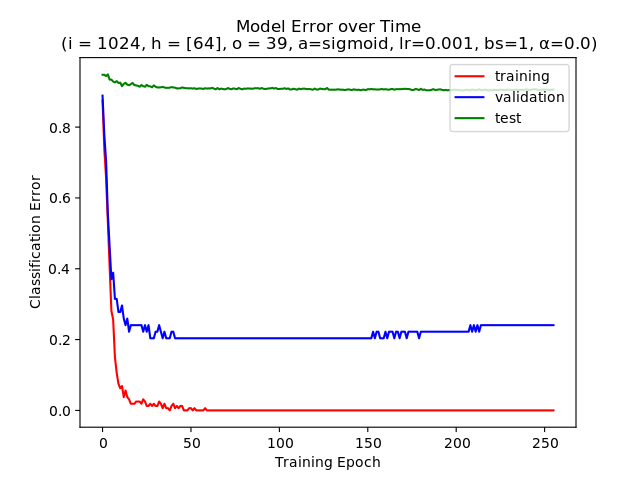
\includegraphics[width=0.5\textwidth]{./img/64-0.001-1-0-sigmoid-1/error-255.png}
      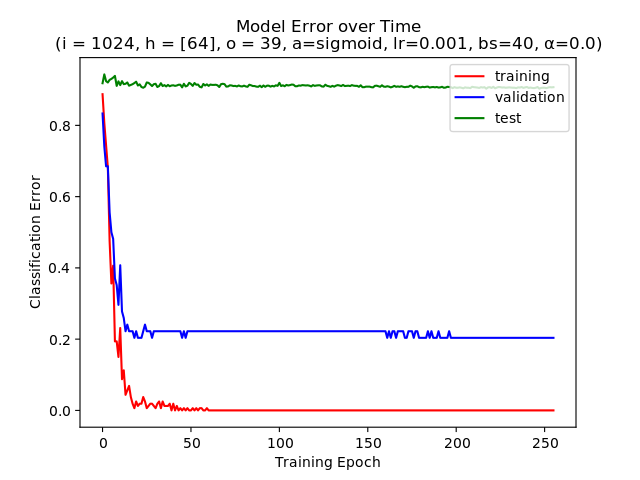
\includegraphics[width=0.5\textwidth]{./img/64-0.001-40-0-sigmoid-1/error-255.png}
      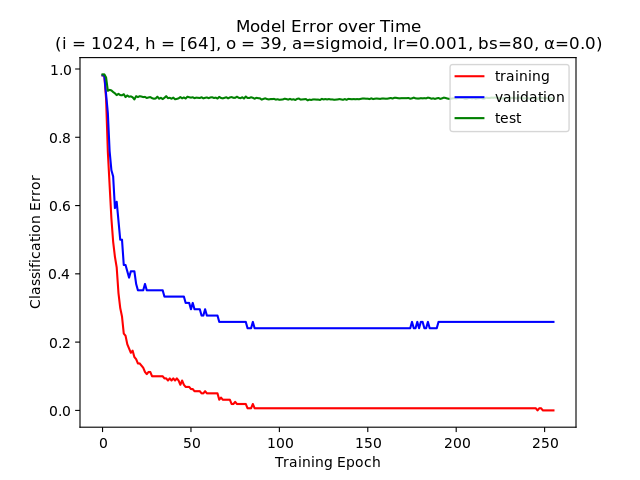
\includegraphics[width=0.5\textwidth]{./img/64-0.001-80-0-sigmoid-1/error-255.png}
      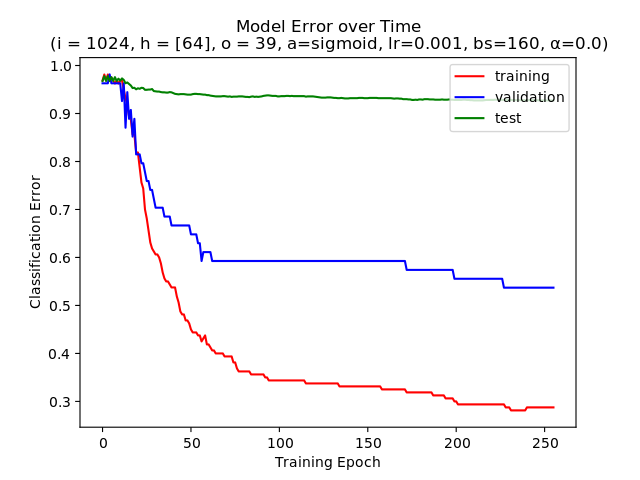
\includegraphics[width=0.5\textwidth]{./img/64-0.001-160-0-sigmoid-1/error-255.png}
      \caption{Classification Errors Varied by Batch Size}
      \label{fig:error-by-b}
    \end{figure}
    \begin{figure}[H]
      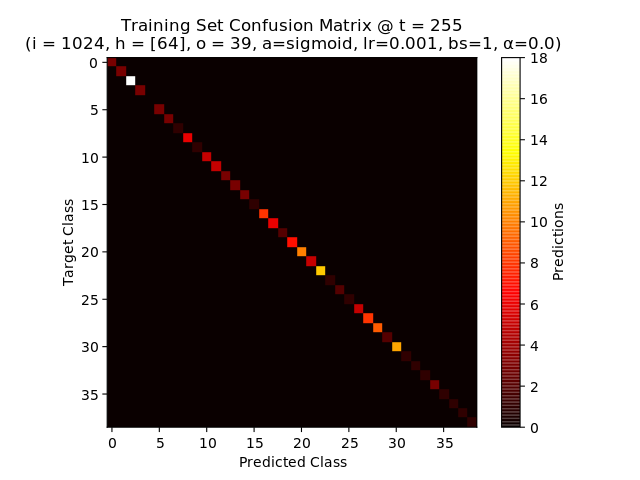
\includegraphics[width=0.33\textwidth]{./img/64-0.001-1-0-sigmoid-1/confusion-matrix-training-255.png}
      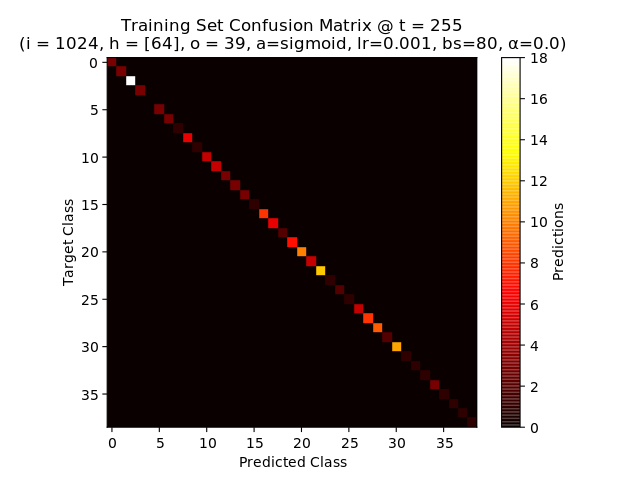
\includegraphics[width=0.33\textwidth]{./img/64-0.001-80-0-sigmoid-1/confusion-matrix-training-255.png}
      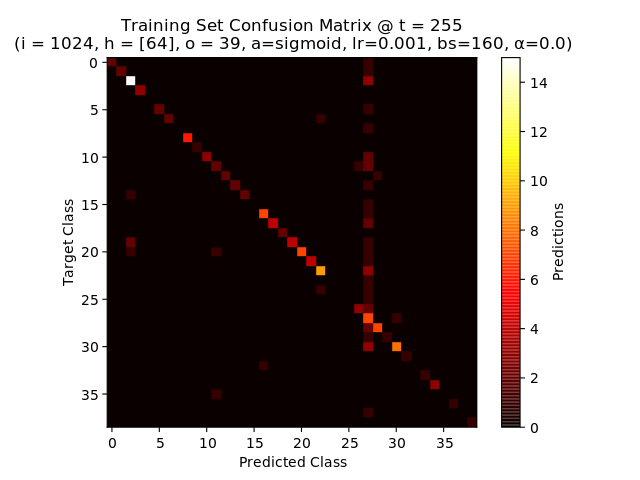
\includegraphics[width=0.33\textwidth]{./img/64-0.001-160-0-sigmoid-1/confusion-matrix-training-255.png}
      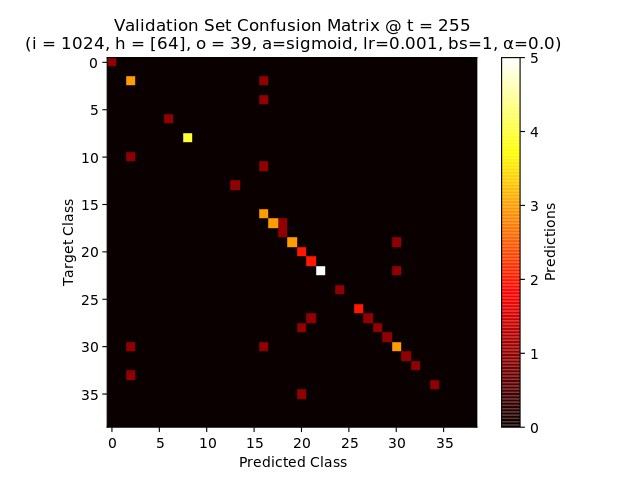
\includegraphics[width=0.33\textwidth]{./img/64-0.001-1-0-sigmoid-1/confusion-matrix-validation-255.png}
      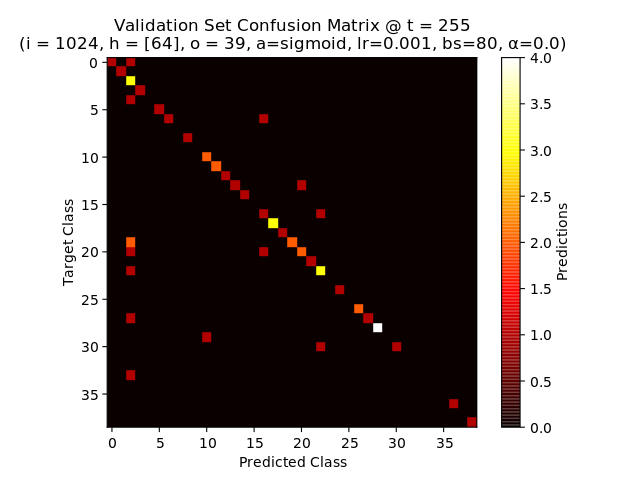
\includegraphics[width=0.33\textwidth]{./img/64-0.001-80-0-sigmoid-1/confusion-matrix-validation-255.png}
      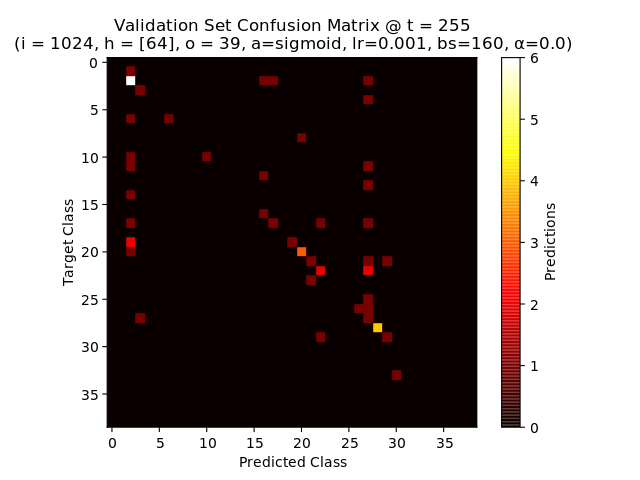
\includegraphics[width=0.33\textwidth]{./img/64-0.001-160-0-sigmoid-1/confusion-matrix-validation-255.png}
      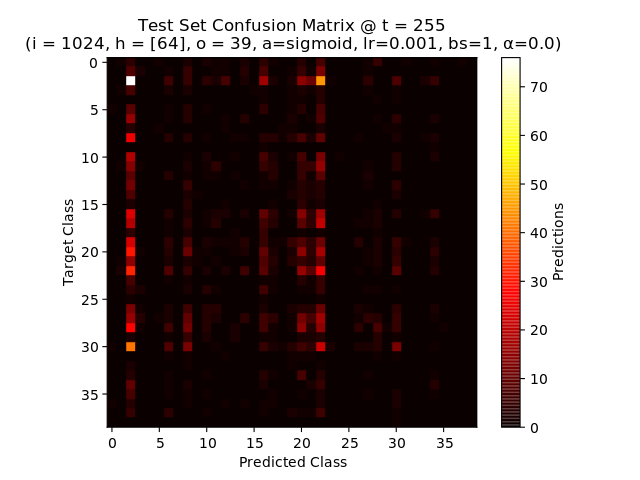
\includegraphics[width=0.33\textwidth]{./img/64-0.001-1-0-sigmoid-1/confusion-matrix-test-255.png}
      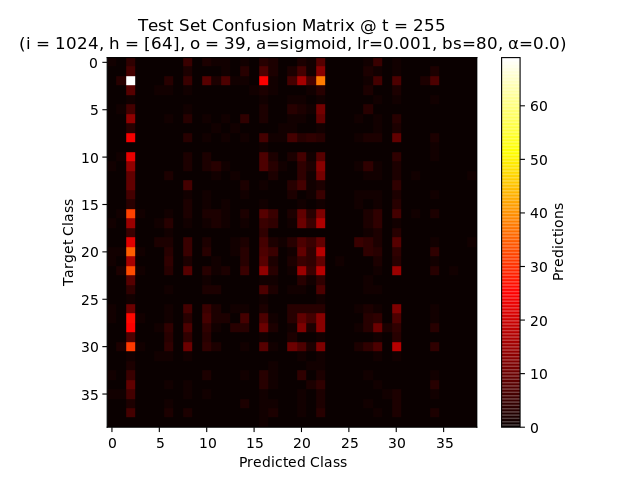
\includegraphics[width=0.33\textwidth]{./img/64-0.001-80-0-sigmoid-1/confusion-matrix-test-255.png}
      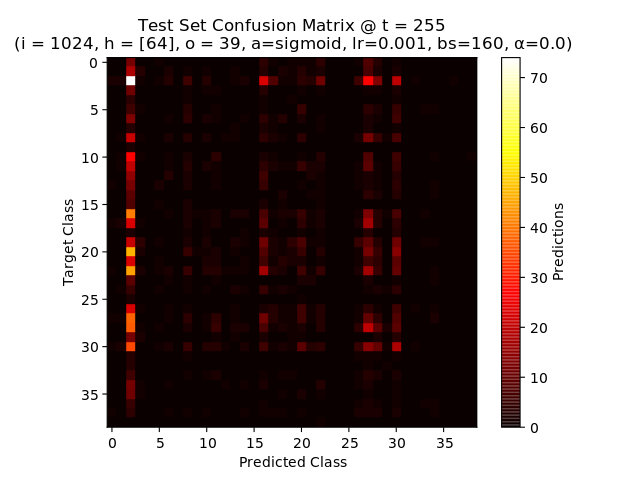
\includegraphics[width=0.33\textwidth]{./img/64-0.001-160-0-sigmoid-1/confusion-matrix-test-255.png}
      \caption{Confusion Matrices Varied by Batch Size}
      \label{fig:cm-by-b}
    \end{figure}
    \paragraph{Variation in $\lambda$}{
      Varying the learning rate led to numerical instability for values greater than 0.001.
      Attempts were made to made to mitigate this, but there is a systemic issue in play here
      that requires more in-depth investigation. Consequently, the plots for weight changes
      and activations observed by varying the learning rate were not captured and are omitted
      from later sections.

      As expected, the intermediate stages witnessed
      a slower decay in error than that observed in the baseline learning rate $\lambda = 0.001$
      The confusion matrices from the last commonly plotted iteration in Fig~\ref{fig:cm-by-lr}
      suffice for illustration.

      The training runs with faster learning rates get quickly wedged in a local minimum that
      reflects a major statistical frequency in the training data. The case $\lambda = 0.01$
      still has echoes of the more common class priors inducing errors by their prevalence,
      but a diagonal is beginning to at least emerge on the training and validation confusion
      matrices. The other cases are unlikely to escape the majority class, which may go toward
      explaining the numerical errors observed that prevented completion of those training runs.
    }
    \begin{figure}[H]
      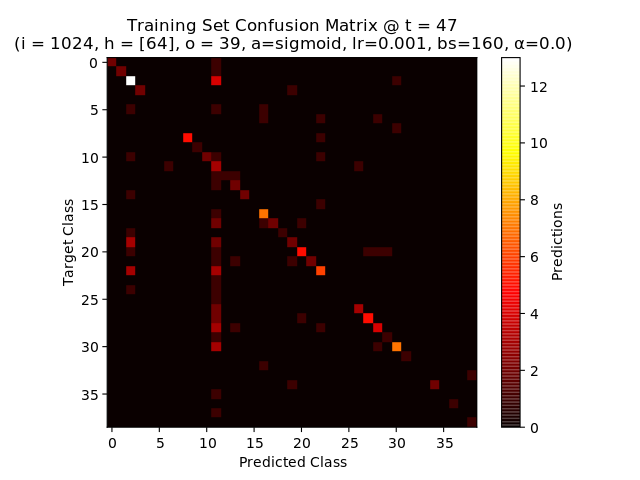
\includegraphics[width=0.33\textwidth]{./img/64-0.001-160-0-sigmoid-1/confusion-matrix-training-47.png}
      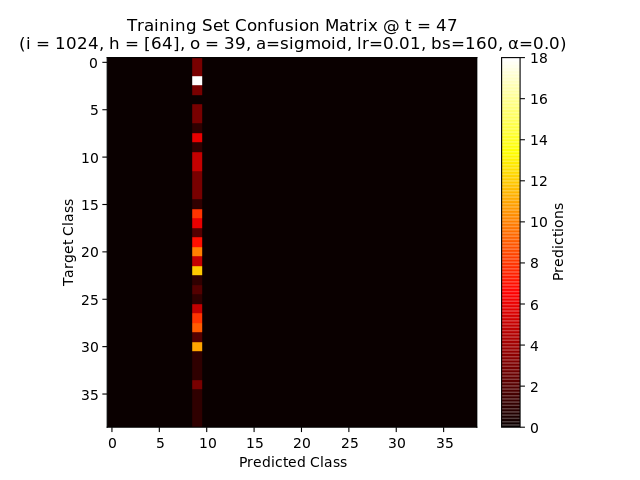
\includegraphics[width=0.33\textwidth]{./img/64-0.01-160-0-sigmoid-1/confusion-matrix-training-47.png}
      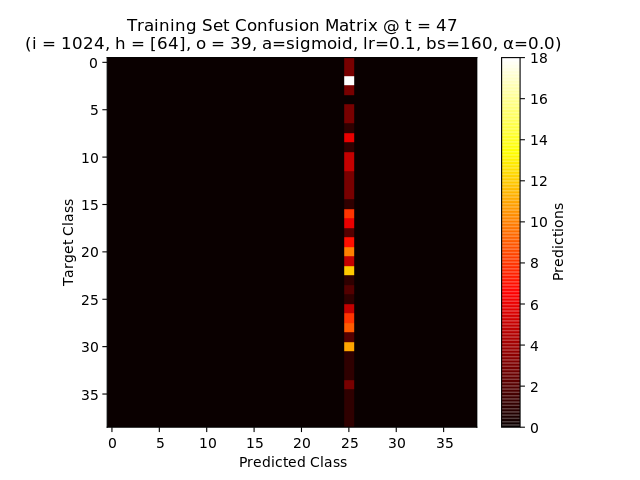
\includegraphics[width=0.33\textwidth]{./img/64-0.1-160-0-sigmoid-1/confusion-matrix-training-47.png}
      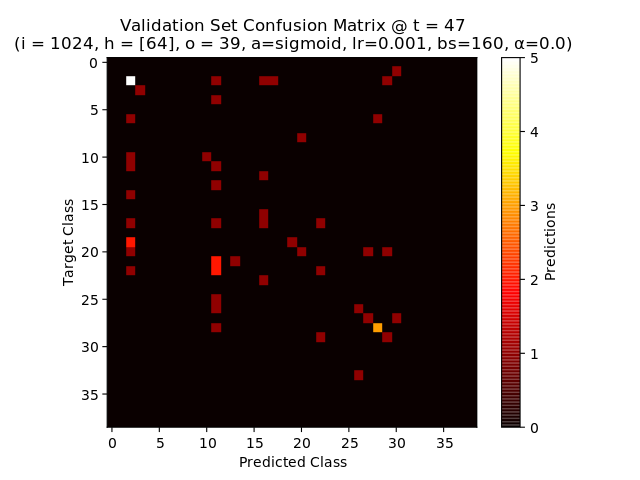
\includegraphics[width=0.33\textwidth]{./img/64-0.001-160-0-sigmoid-1/confusion-matrix-validation-47.png}
      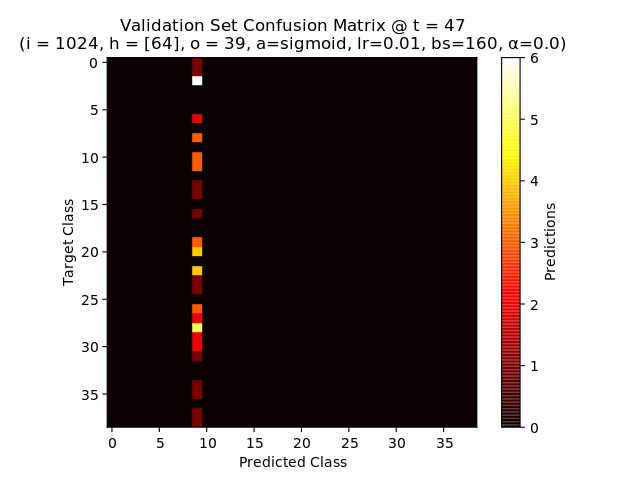
\includegraphics[width=0.33\textwidth]{./img/64-0.01-160-0-sigmoid-1/confusion-matrix-validation-47.png}
      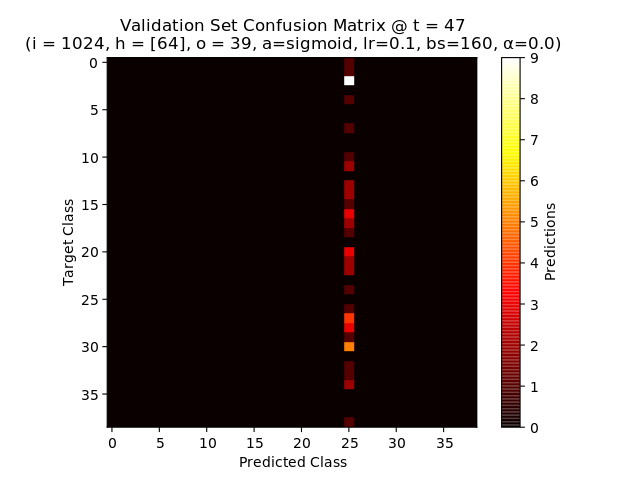
\includegraphics[width=0.33\textwidth]{./img/64-0.1-160-0-sigmoid-1/confusion-matrix-validation-47.png}
      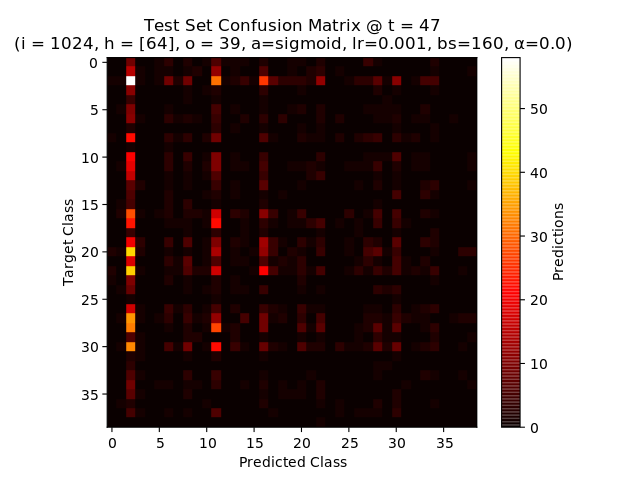
\includegraphics[width=0.33\textwidth]{./img/64-0.001-160-0-sigmoid-1/confusion-matrix-test-47.png}
      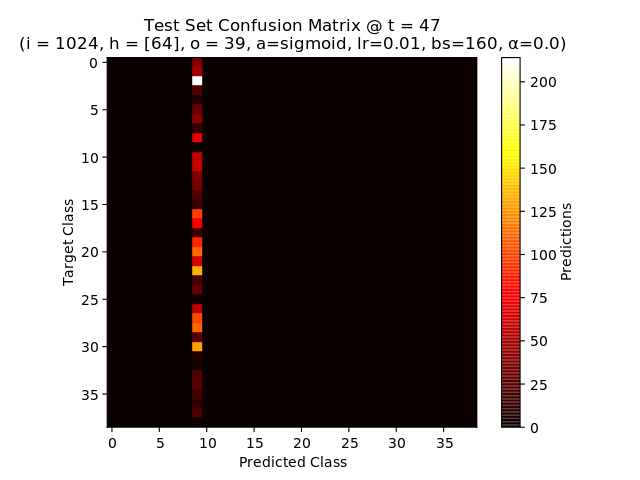
\includegraphics[width=0.33\textwidth]{./img/64-0.01-160-0-sigmoid-1/confusion-matrix-test-47.png}
      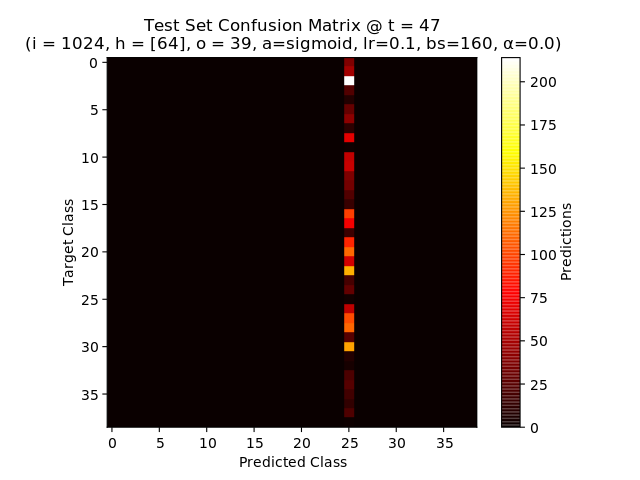
\includegraphics[width=0.33\textwidth]{./img/64-0.1-160-0-sigmoid-1/confusion-matrix-test-47.png}
      \caption{Confusion Matrices Varied by Learning Rate}
      \label{fig:cm-by-lr}
    \end{figure}
    \paragraph{Variation in $N_H$}{
      Fig~\ref{fig:error-by-nh} illustrates the variation in error resulting from a change in
      node count for the hidden layer. The lower, less expressive node counts appear to
      introduce significant jitter in the evolution of the error metric. This makes intuitive
      sense since a weight change in a single node has a greater potential impact on the hidden
      layer output when the nodes are few. There are fewer counterweights to counteract the mistakes
      of one hidden node. The lower count cases also reach the overfitting point much more quickly.
      There appears to be a linear relationship between the inflection point and the number of
      nodes. Assume a function $f$ that maps node count to the inflection epoch, i.e.,
      $f(N_H) = t_{overfit}$.
      In these examples, $f(1) \approx 75, f(4) \approx 100, f(16) \approx 175, f(64) > 256$.
    }
    \begin{figure}[H]
      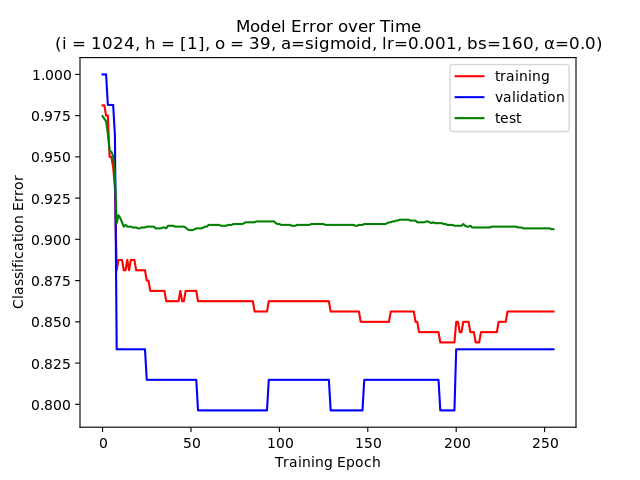
\includegraphics[width=0.5\textwidth]{./img/1-0.001-160-0-sigmoid-1/error-255.png}
      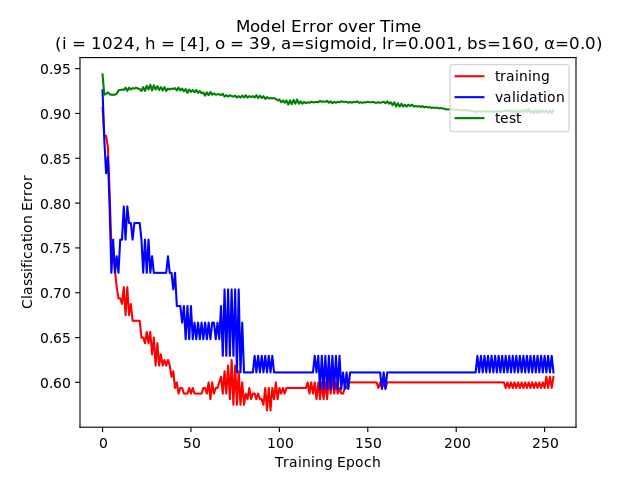
\includegraphics[width=0.5\textwidth]{./img/4-0.001-160-0-sigmoid-1/error-255.png}
      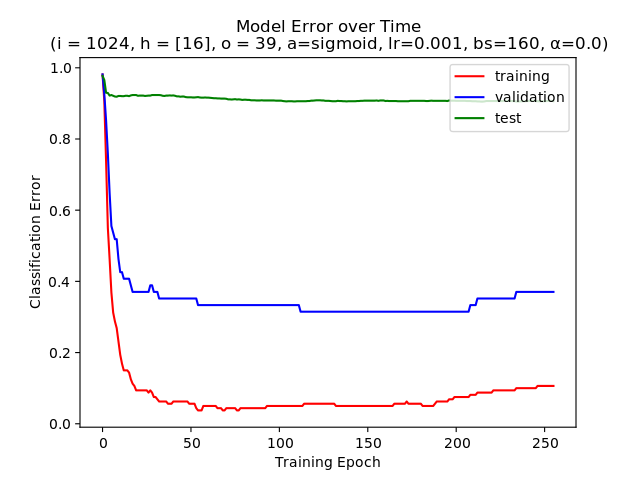
\includegraphics[width=0.5\textwidth]{./img/16-0.001-160-0-sigmoid-1/error-255.png}
      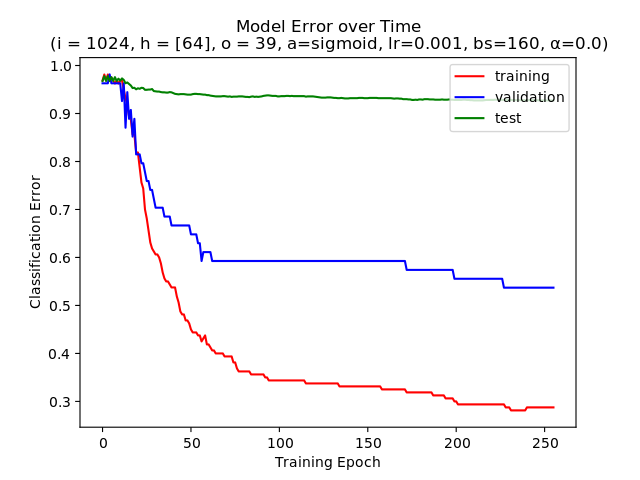
\includegraphics[width=0.5\textwidth]{./img/64-0.001-160-0-sigmoid-1/error-255.png}
      \caption{Classification Errors Varied by Hidden Layer Node Count}
      \label{fig:error-by-nh}
    \end{figure}
    \paragraph{Variation in $\alpha$}{
      Fig~\ref{fig:error-by-m} illustrates the variation in error resulting from a change in
      momentum. From the juxtaposition of images, the momentum appears to have an inversely
      proportional relationship with stability, in keeping with its ostensible use as a means
      of overcoming plateaus in learning.

      The \emph{effect} could be compared to that observed from the constant reintroduction of a catalyst
      into a system so that the reagents never reach equilibrium, but ironically the \emph{cause} is the
      diametric opposite. By dampening the weight changes, the system fails to converge quickly
      and follows a harmonic attenuation towards what is presumably an equilibrium state.
      The most textbook case of this is observed when $\alpha = 0.9$, which is unsurprisingly
      the value asserted as typical by Duda, Hart, and Stork in their text\autocite[314]{DHS}.

      Disappointingly, the final accuracy, even in the test set, is rather lower than what
      was observed for training with no momentum. Whatever local minima it may have avoided,
      the training with momentum seems to have settled on a suboptimal local minimum of its own.

      The confusion matrices depicted in Fig~\ref{fig:cm-by-m} underscore the poor performance
      caused by adding momentum, particularly when $\alpha = 1.0$. The majority classes dominate
      more as momentum is increased, at least for the 256 epochs observed.
    }
    \begin{figure}[H]
      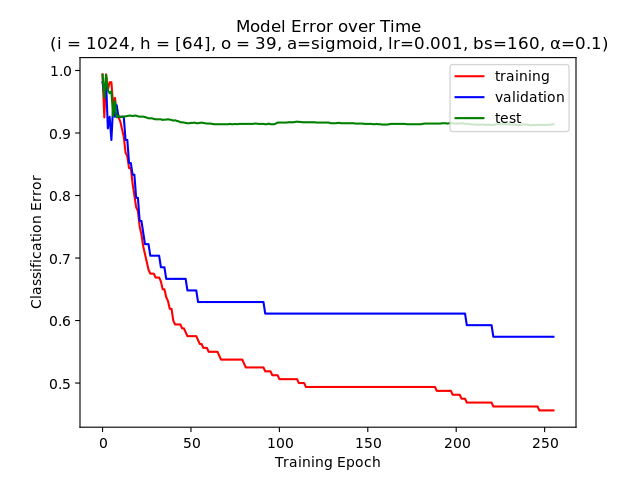
\includegraphics[width=0.5\textwidth]{./img/64-0.001-160-0.1-sigmoid-1/error-255.png}
      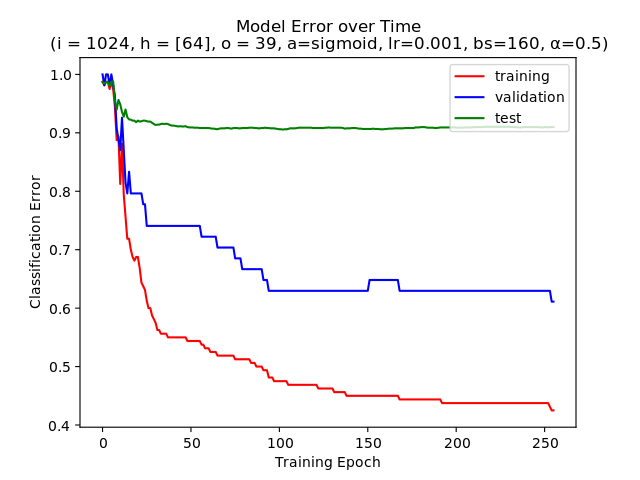
\includegraphics[width=0.5\textwidth]{./img/64-0.001-160-0.5-sigmoid-1/error-255.png}
      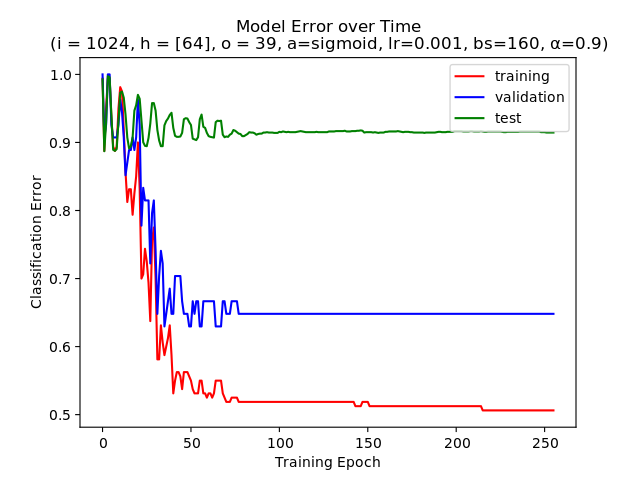
\includegraphics[width=0.5\textwidth]{./img/64-0.001-160-0.9-sigmoid-1/error-255.png}
      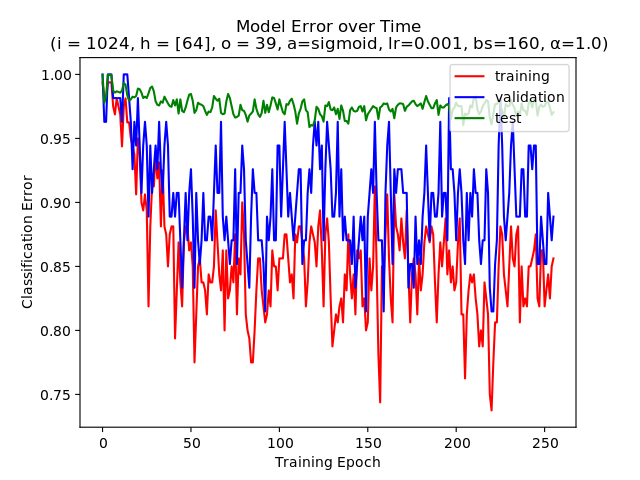
\includegraphics[width=0.5\textwidth]{./img/64-0.001-160-1-sigmoid-1/error-255.png}
      \caption{Classification Errors Varied by Momentum}
      \label{fig:error-by-m}
    \end{figure}
    \begin{figure}[H]
      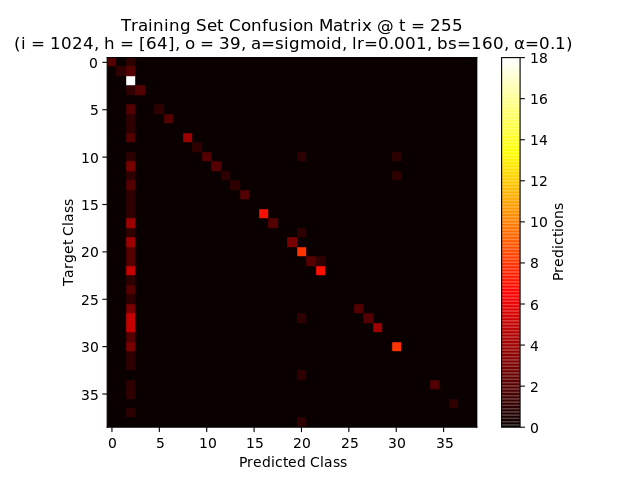
\includegraphics[width=0.33\textwidth]{./img/64-0.001-160-0.1-sigmoid-1/confusion-matrix-training-255.png}
      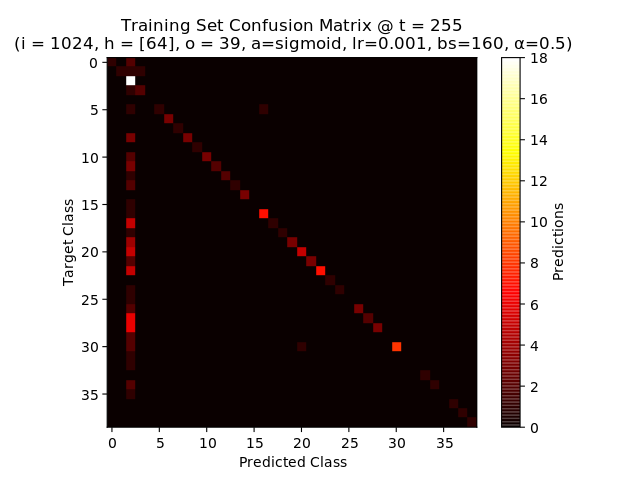
\includegraphics[width=0.33\textwidth]{./img/64-0.001-160-0.5-sigmoid-1/confusion-matrix-training-255.png}
      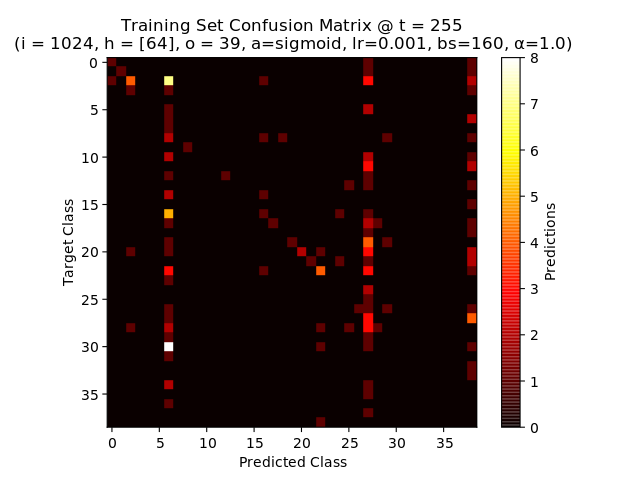
\includegraphics[width=0.33\textwidth]{./img/64-0.001-160-1-sigmoid-1/confusion-matrix-training-255.png}
      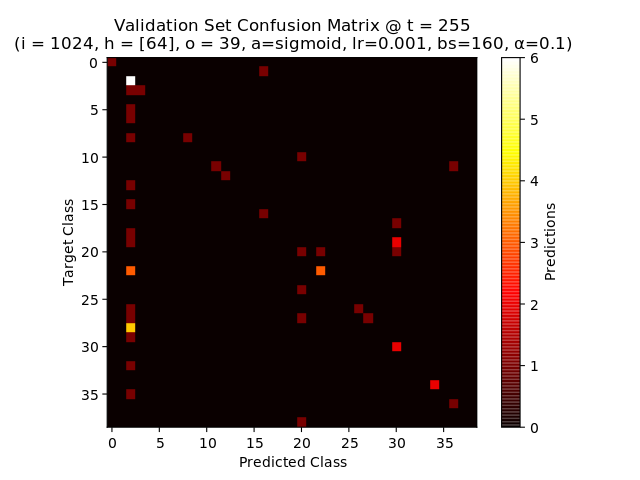
\includegraphics[width=0.33\textwidth]{./img/64-0.001-160-0.1-sigmoid-1/confusion-matrix-validation-255.png}
      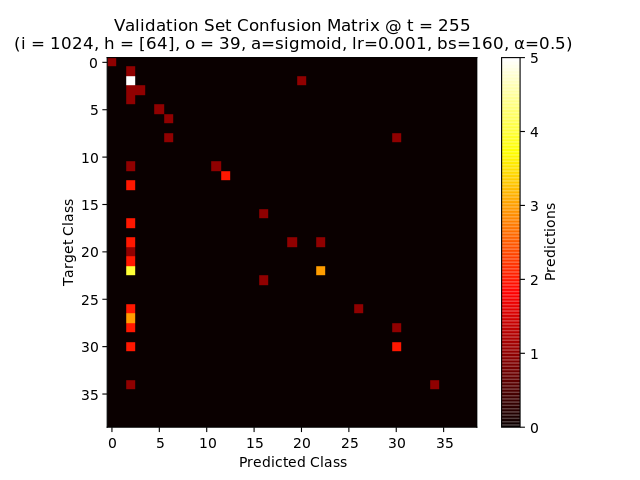
\includegraphics[width=0.33\textwidth]{./img/64-0.001-160-0.5-sigmoid-1/confusion-matrix-validation-255.png}
      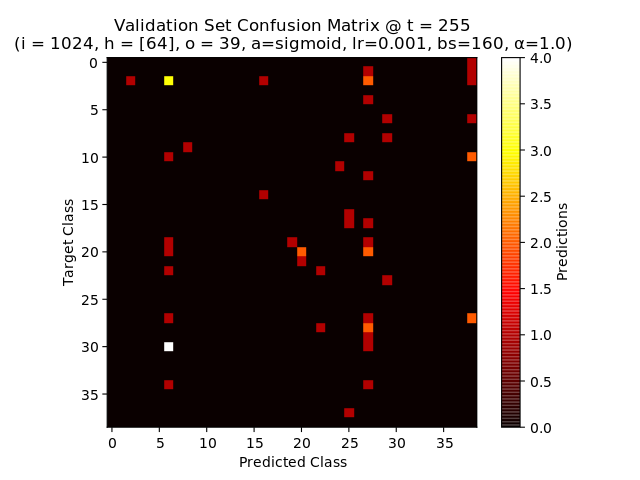
\includegraphics[width=0.33\textwidth]{./img/64-0.001-160-1-sigmoid-1/confusion-matrix-validation-255.png}
      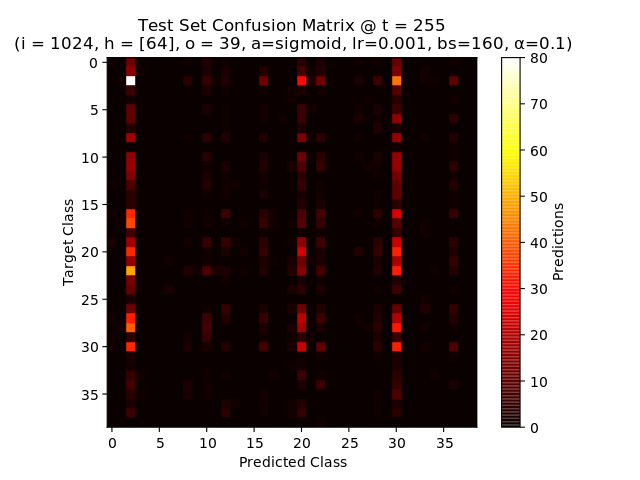
\includegraphics[width=0.33\textwidth]{./img/64-0.001-160-0.1-sigmoid-1/confusion-matrix-test-255.png}
      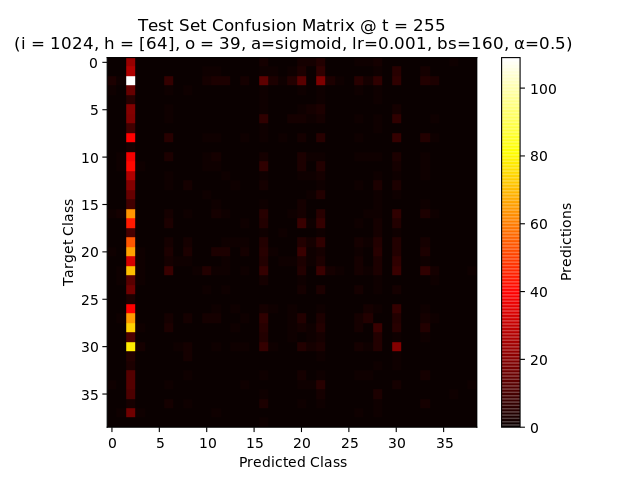
\includegraphics[width=0.33\textwidth]{./img/64-0.001-160-0.5-sigmoid-1/confusion-matrix-test-255.png}
      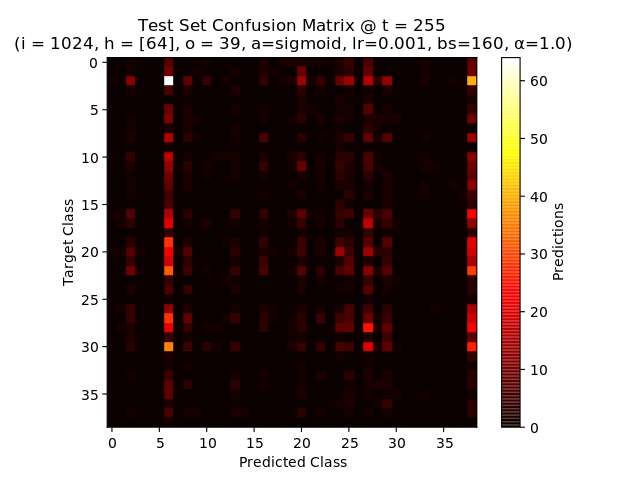
\includegraphics[width=0.33\textwidth]{./img/64-0.001-160-1-sigmoid-1/confusion-matrix-test-255.png}
      \caption{Confusion Matrices Varied by Momentum}
      \label{fig:cm-by-m}
    \end{figure}
    \paragraph{Variation in $u$}{
      Fig~\ref{fig:error-by-u} illustrates the variation in error resulting from a change in
      non-linear activation unit. The hyperbolic tangent easily outstrips the sigmoid in
      overfitting the training set in what appears to be approximately only 20 epochs.
      Of the regimens, $\tanh$ appears to be the most stable and consequently the most
      impervious to improvement. The validation and test accuracy is significantly better
      compared with the sigmoid in the same cohort, but better results were achieved in
      Fig~\ref{fig:error-by-b} by smaller batch sizes.

      The ReLU activation function appears to provide the best absolute accuracy on the
      validation set, but it clearly begins to overfit around epoch 150. It also appears
      to undergo periods of jitter where the weights are perhaps vacillating in response
      to the training sample order permutations.
    }
    \begin{figure}[H]
      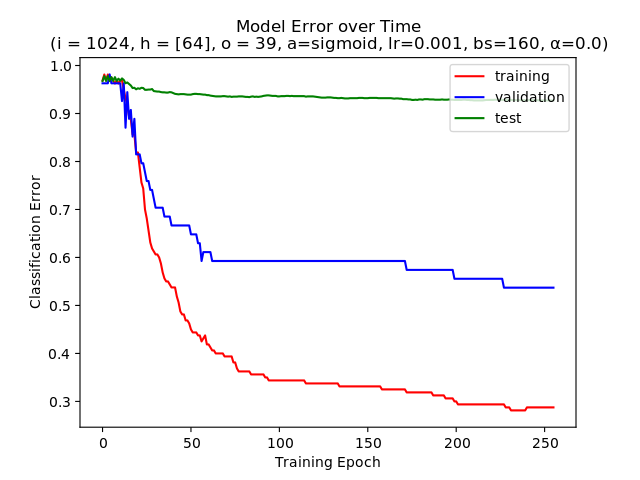
\includegraphics[width=0.5\textwidth]{./img/64-0.001-160-0-sigmoid-1/error-255.png}
      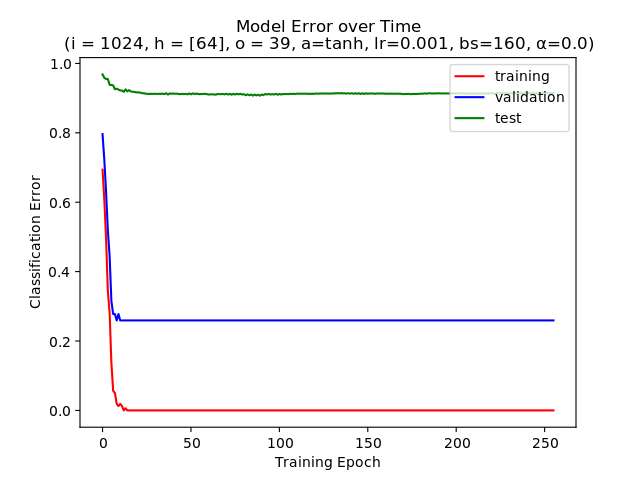
\includegraphics[width=0.5\textwidth]{./img/64-0.001-160-0-tanh-1/error-255.png}
      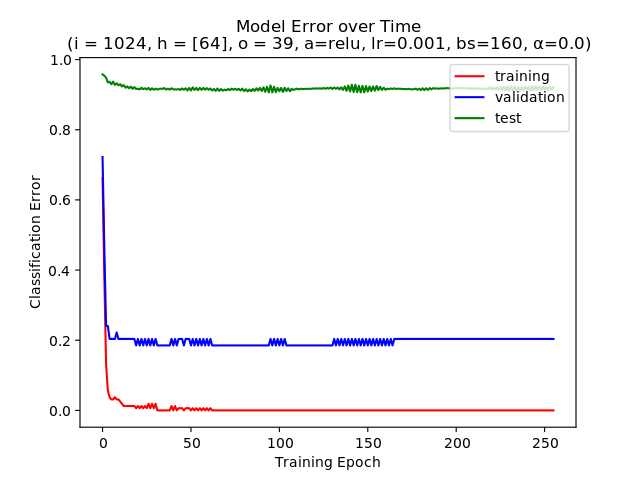
\includegraphics[width=0.5\textwidth]{./img/64-0.001-160-0-relu-1/error-255.png}
      \caption{Classification Errors Varied by Activation Unit}
      \label{fig:error-by-u}
    \end{figure}
  }
  \subsection{Changes in Weight Over Time}{
    To plot changes in layer weights over the training cycle, a heatmap was adopted to simultaneously
    illustrate the changes for all layers in a single concise graphic. A frequent  observation was
    that the weight changes quickly rose in a crescendo in the first few epochs of training and then
    quickly dropped off and stabilized. The classification error follows a similar enough pattern that
    the error graph might appear proportional to a cross-section of the weight change heat map
    if it were extruded into three-dimensional space. Plots for weight vector norm difference per epoch
    were created, but they are omitted here as the information is redundant with the angle delta plots.
    \paragraph{Variation in $b$}{
      Fig~\ref{fig:dw-by-b} illustrates the weight change history for variations in batch size.
      As batch size increases, the weight changes become more gradual and less pronounced. This follows
      intuitively since smaller batch sizes incur opportunities for more immediate backpropagation
      multiple times within an epoch. As such, the model changes to fit each sample, becoming quicker
      to overfit as the batch size decreases.
    }
    \begin{figure}[H]
      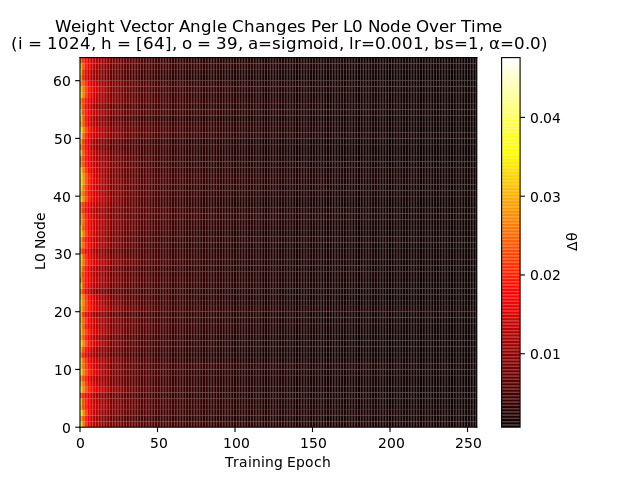
\includegraphics[width=0.5\textwidth]{./img/64-0.001-1-0-sigmoid-1/weight-angle-changes-L0-255.png}
      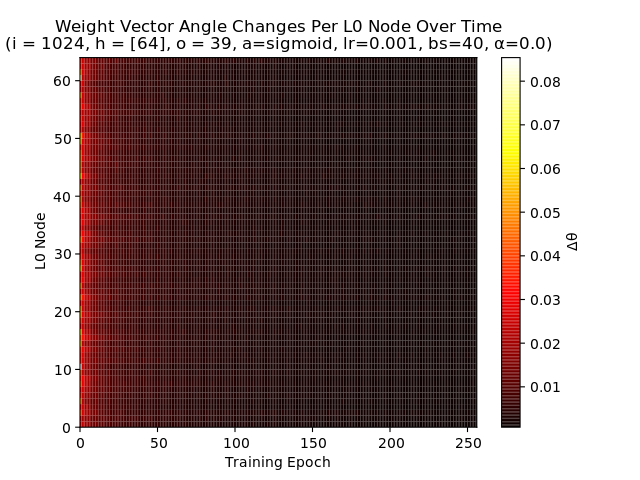
\includegraphics[width=0.5\textwidth]{./img/64-0.001-40-0-sigmoid-1/weight-angle-changes-L0-255.png}
      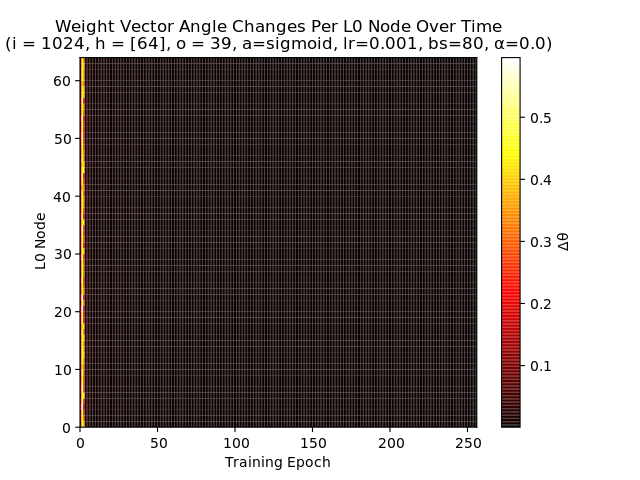
\includegraphics[width=0.5\textwidth]{./img/64-0.001-80-0-sigmoid-1/weight-angle-changes-L0-255.png}
      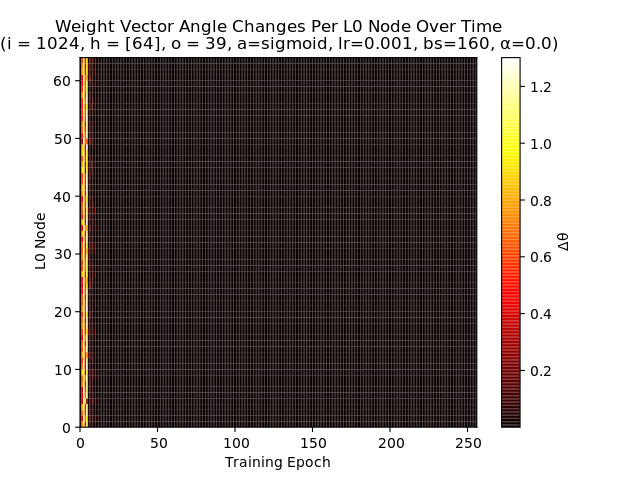
\includegraphics[width=0.5\textwidth]{./img/64-0.001-160-0-sigmoid-1/weight-angle-changes-L0-255.png}
      \caption{Weight Vector Changes Varied by Batch Size}
      \label{fig:dw-by-b}
    \end{figure}
    \paragraph{Variation in $N_H$}{
      Fig~\ref{fig:dw-by-nh} illustrates the weight change history for variations in hidden node count.
      With a single hidden node, the weight changes appear relatively small for the most part, although
      some of that may be an issue with artifacting in matplotlib that is masking the ostensible maxima.
      With four hidden nodes, it appears that nodes 0 and 2 incur the most sustained change over time,
      while nodes 1 and 3 remain relatively quiescent. As node count increases, the majority of the time
      is spent making minor adjustments with a burst of change in the early epochs. The burst is more
      pronounced in the $N_H = 64$ both in relative and absolute magnitude.
    }
    \begin{figure}[H]
      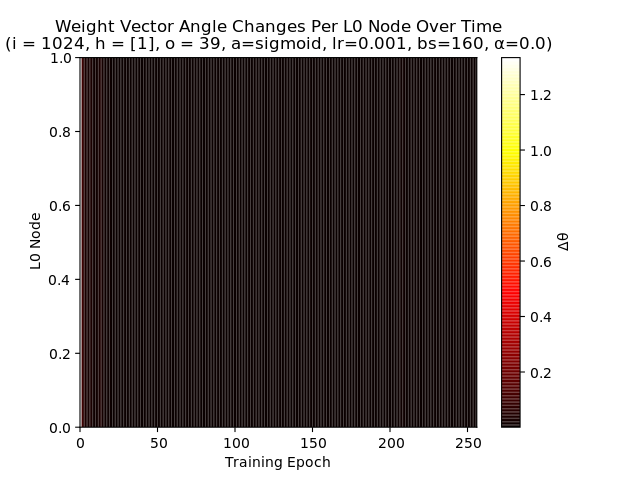
\includegraphics[width=0.5\textwidth]{./img/1-0.001-160-0-sigmoid-1/weight-angle-changes-L0-255.png}
      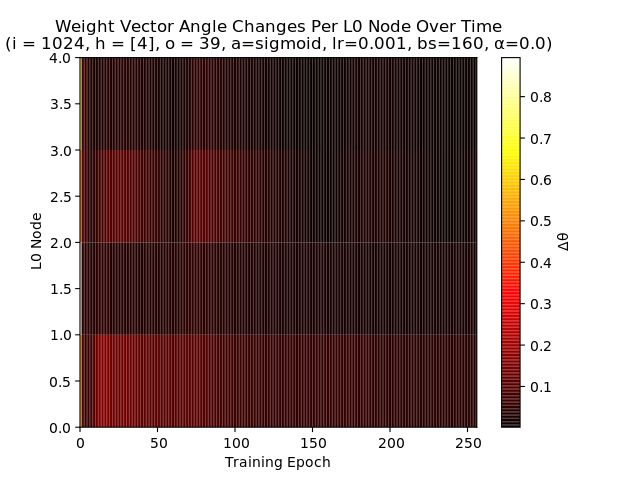
\includegraphics[width=0.5\textwidth]{./img/4-0.001-160-0-sigmoid-1/weight-angle-changes-L0-255.png}
      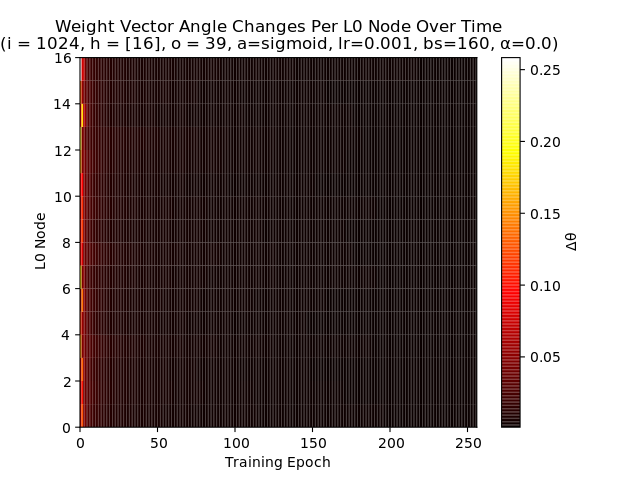
\includegraphics[width=0.5\textwidth]{./img/16-0.001-160-0-sigmoid-1/weight-angle-changes-L0-255.png}
      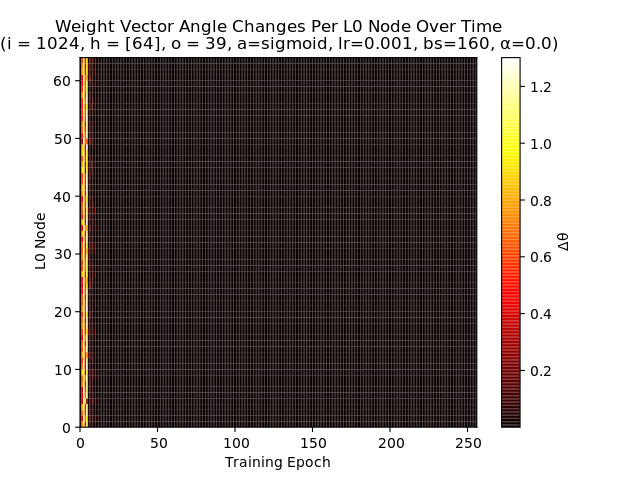
\includegraphics[width=0.5\textwidth]{./img/64-0.001-160-0-sigmoid-1/weight-angle-changes-L0-255.png}
      \caption{Weight Vector Changes Varied by Hidden Layer Node Count}
      \label{fig:dw-by-nh}
    \end{figure}
    \paragraph{Variation in $\alpha$}{
      Fig~\ref{fig:dw-by-m} illustrates the weight change history for variations in momentum.
      There is little than can be remarked on with respect to the
      changes due to momentum given the controls for the other model parameters. The graph is
      essentially indistinguishable from the same graph in Fig~\ref{fig:dw-by-b} where the batch size,
      hidden node count, learning rate, and activation unit match. It may be that there are observable
      differences under different parameter control cohorts, but these were not explored on account
      of time and available computational resources.
    }
    \begin{figure}[H]
      \includegraphics[width=0.5\textwidth]{./img/64-0.001-160-0.1-sigmoid-1/weight-angle-changes-L0-255.png}
      \includegraphics[width=0.5\textwidth]{./img/64-0.001-160-0.5-sigmoid-1/weight-angle-changes-L0-255.png}
      \includegraphics[width=0.5\textwidth]{./img/64-0.001-160-0.9-sigmoid-1/weight-angle-changes-L0-255.png}
      \includegraphics[width=0.5\textwidth]{./img/64-0.001-160-1-sigmoid-1/weight-angle-changes-L0-255.png}
      \caption{Weight Vector Changes Varied by Momentum}
      \label{fig:dw-by-m}
    \end{figure}
    \paragraph{Variation in $u$}{
      Fig~\ref{fig:dw-by-u} illustrates the weight change history for variations in activation unit.
      The weight changes under the hyperbolic tangent are more
      diffused than under the sigmoid, though the scale is appreciably smaller -- by more than half.
      The reduction in scale does permit a glimpse at distinguishing the weight changes over time
      across different nodes. What appears in the sigmoid to be uniform across the whole layer
      seems in the sigmoid to vary in decay with a few choice nodes undergoing an extended trail
      of revisions while most nodes go quiescent around the time of the inflection toward
      stabilization in the training set.

      The ReLU activation function presents the most consistent fluctuation over time in the weights
      and resembles a seismograph or a spectrogram when plotting the respective nodes against time.
      The dynamic range is also smaller than for the sigmoid or tanh activation functions, and seems
      to support a notion of behavior that makes many small tweaks over time versus the bursty nature
      of the sigmoid with respect to weight change.
    }
    \begin{figure}[H]
      \includegraphics[width=0.5\textwidth]{./img/64-0.001-160-0-sigmoid-1/weight-angle-changes-L0-255.png}
      \includegraphics[width=0.5\textwidth]{./img/64-0.001-160-0-tanh-1/weight-angle-changes-L0-255.png}
      \includegraphics[width=0.5\textwidth]{./img/64-0.001-160-0-relu-1/weight-angle-changes-L0-255.png}
      \caption{Weight Vector Changes Varied by Activation}
      \label{fig:dw-by-u}
    \end{figure}
  }

  \subsection{Non-Linear Activations}{
    \paragraph{Variation in $b$}{
      Fig~\ref{fig:a-by-b} illustrates the output of the activation unit for each hidden input node
      over variations in batch size. When batch size is small, the distribution of activations
      appears to follow a normal distribution with mean at 0.5. As batch size increases, this
      gradually morphs into a bimodal distribution with peaks at 0 and 1. The distribution
      appear to be consistent across multiple nodes. The larger peak occurs around zero (0),
      which makes sense since the model is likely concentrating its ``voting power'' in the
      learned class outputs and zeroing out most others.
    }
    \begin{figure}[H]
      \includegraphics[width=0.5\textwidth]{./img/64-0.001-1-0-sigmoid-1/activations-A0-255.png}
      \includegraphics[width=0.5\textwidth]{./img/64-0.001-40-0-sigmoid-1/activations-A0-255.png}
      \includegraphics[width=0.5\textwidth]{./img/64-0.001-80-0-sigmoid-1/activations-A0-255.png}
      \includegraphics[width=0.5\textwidth]{./img/64-0.001-160-0-sigmoid-1/activations-A0-255.png}
      \caption{Activations Varied by Batch Size}
      \label{fig:a-by-b}
    \end{figure}
    \paragraph{Variation in $N_H$}{
      Fig~\ref{fig:a-by-nh} illustrates the output of the activation unit for each hidden input node
      over variations in hidden node count. The extrema in node count exhibit the bimodal distribution
      seen previously in the large batch size while the middle counts are closer to the normal
      distribution. The case where $N_H = 4$ appears to be more disorganized in its distribution
      than where $N_H = 16$, though this appears to correlate to the weight vector changes observed.

      This suggests that a node subject to more emphatic swings in its weights over longer periods of
      time will reflect this in the form of a normal random activation pattern, while nodes which remain
      relatively cool will settle into a stable bimodal pattern. This may also correlate with
      the overfitting inflection point, which does not appear to be reached in the case where $N_H = 64$.

      It should be noted that the $N_H = 1$, while bimodal, has a more gradual slope than $N_H = 64$.
      This supports the prior supposition that extended jitter diffuses the activations over a wider
      area. The single node case may also be exhibiting some degeneracy by virtue of it having to compress
      a 39-class decision into a single scalar that is then weighted accordingly by the output layer.
    }
    \begin{figure}[H]
      \includegraphics[width=0.5\textwidth]{./img/1-0.001-160-0-sigmoid-1/activations-A0-255.png}
      \includegraphics[width=0.5\textwidth]{./img/4-0.001-160-0-sigmoid-1/activations-A0-255.png}
      \includegraphics[width=0.5\textwidth]{./img/16-0.001-160-0-sigmoid-1/activations-A0-255.png}
      \includegraphics[width=0.5\textwidth]{./img/64-0.001-160-0-sigmoid-1/activations-A0-255.png}
      \caption{Activations Varied by Hidden Layer Node Count}
      \label{fig:a-by-nh}
    \end{figure}
    \paragraph{Variation in $\alpha$}{
      Fig~\ref{fig:a-by-m} illustrates the output of the activation unit for each hidden input node
      over variations in momentum. The bimodal distribution of the comparable zero-momentum case
      is here preserved. What is interesting is the inversion of major and minor peaks when
      $\alpha = 1.0$. The discrepancy is not as large compared to the other cases, but the strong
      activations take precedence over the weak activations. The noisiness of the corresponding
      error graph in Fig~\ref{fig:error-by-m} provides a clue: with $\alpha = 1.0$, the model never
      settles enough to confidently activate one node or a small handful of nodes in the output
      layer and leave the rest quiet as a mature model might. With the best accuracy
      \emph{in the training set} briefly courting 25 percent, the model has simply not progressed enough.
    }
    \begin{figure}[H]
      \includegraphics[width=0.5\textwidth]{./img/64-0.001-160-0.1-sigmoid-1/activations-A0-255.png}
      \includegraphics[width=0.5\textwidth]{./img/64-0.001-160-0.5-sigmoid-1/activations-A0-255.png}
      \includegraphics[width=0.5\textwidth]{./img/64-0.001-160-0.9-sigmoid-1/activations-A0-255.png}
      \includegraphics[width=0.5\textwidth]{./img/64-0.001-160-1-sigmoid-1/activations-A0-255.png}
      \caption{Activations Varied by Momentum}
      \label{fig:a-by-m}
    \end{figure}
    \paragraph{Variation in $u$}{
      Fig~\ref{fig:a-by-u} illustrates the output of the activation unit for each hidden input node
      over variations in activation unit. The difference between the sigmoid and hyperbolic tangent
      is striking. While the sigmoid shows the bimodal distribution that suggests a confidence
      in output, $\tanh$ exhibits a nearly uniform distribution in activations, or at least a
      normal distribution with a high variance and not much representation at the extrema. One is
      left to wonder whether the performance of the hyperbolic tangent is truly good even at overfitting
      or if random chance played a significant role in selecting the right argmax values. A more
      rigorous study might help suss out the answer to these questions.

      The ReLU plot shows an overwhelming preference for activations in the highest bin. This is
      an artifact of the implementation that includes some information loss. The ReLU function
      simply clamps negative values to zero but provides no upper bound. The plotting mechanism
      assumed a range of $[0,1]$, and so several test runs crashed \emph{in medias res}. The quickest
      fix was to clamp copies of the activation tensors used for plotting to an upper bound of 1,
      so the last bin technically represents any activation greater than 0.95. The ReLU function
      also distributes more heat to the lower bins than the sigmoid, though not as evenly as the
      hyperbolic tangent.
    }
    \begin{figure}[H]
      \includegraphics[width=0.5\textwidth]{./img/64-0.001-160-0-sigmoid-1/activations-A0-255.png}
      \includegraphics[width=0.5\textwidth]{./img/64-0.001-160-0-tanh-1/activations-A0-255.png}
      \includegraphics[width=0.5\textwidth]{./img/64-0.001-160-0-relu-1/activations-A0-255.png}
      \caption{Activations Varied by Activation}
      \label{fig:a-by-u}
    \end{figure}
  }
}
\section{Conclusions}{
  Although the experiments were undertaken in the spirit of the Phoneme challenge presented by
  the University of East Anglia, the methodology of learning against a training set so small,
  particularly one dwarfed by the corresponding test set, was never likely to yield any notable accuracy.
  Most of the phoneme classes only included 4 samples while a few predominant phonemes had
  significantly higher populations, e.g., 18.

  Further, a data-naive application of neural networks is only valuable insofar as the training set
  precisely captures the statistical relationship between the input features in reality and that
  these selfsame statistical relationships provide a sufficient test statistic for classification.
  The samples used for training came from a sanitized and somewhat ideal corpus, namely the straight
  reading of dictionary words. This could hardly be considered on its face to be strictly representative
  of utterances in the wild. Brief smoke tests of inverting the relationship between test set and training
  set were attempted but did not significantly improve the model's performance compared to a case
  similarly parameterized, e.g.,

  \begin{figure}[H]
    \centering
    \includegraphics[width=0.5\textwidth]{./img/inverted-smoke-test-confusion-matrix.png}
    \caption{Confusion Matrix from Inverting the Training and Test Sets}
    \label{fig:inv-cm}
  \end{figure}

  There is an additional tacit but nonetheless potentially significant factor contributing to overfitting
  in this and similar experiments. The entire corpus from which the phoneme slices are derived is
  in English. Entire classes of phonemes exist which English speakers do not utter in their native tongue
  as lexical constituents, e.g., trills, clicks, implosives, and pharyngeal stops. Even if the
  experiments were moderately successful, any conclusions drawn would be constrained to Anglophonic
  applications.

  In terms of performance, profiling with the standard Python profiling libraries revealed the
  the data-loading and the forward hook for activation histograms as the most time-intensive hotspots.
  Part of the difficulty in expediting the loading of the data is that the ARFF format is not
  conducive to direct ingestion into PyTorch tensors. The naive conversion from a
  heterogeneous numpy array through unzipping and tuple-slicing simply takes an inordinate
  amount of time relative to the training time. Each nominal class label, though technically
  the string representation of a number, had to be decoded from UTF-8 byte encodings.

  The activation heatmap maintained separate bins for each hidden node and had to assign
  each hidden output to its respective bin in the respective node, an operation with cubic
  asymptotic complexity dimensioned by layers, layer nodes, and sample iterations. It might be
  worth investigating whether a row- or column-wise version of the Pytorch \texttt{tensor.histc}
  operation exists that could mitigate some of the looping cost, to say nothing of the forward hook
  overhead. A better design might have been to extend the Sigmoid, ReLU, and Tanh modules with
  innate state for tracking histograms inside the forward override itself.

  Let us assume for the sake of argument that having considered the issues mentioned above that
  the goal is simply to construct a decently performing English phoneme classifier for pre-constrained,
  normalized sample windows. Whereas amplitude values provide the basis for the spectral
  criteria used in most acoustic language processing frameworks, the translation from the time domain
  into the frequency domain requires a convolution of the input. This would be better represented
  through a complete graph of the input nodes as opposed to a mere feedforward network.
  At that point, one may as well compute the Fourier transform, a thoroughly analyzed
  and widely adopted computation specially suited to acoustic modeling, and be done with it rather
  than spend epochs accumulating vast corpora and fiddling uninterpretable parameters.

  Though the answer to the question posited by the title may appear self-evident, the experiments
  undertaken provided an opportunity for a data-driven discourse in the applicability of neural
  networks and the dangers of using them indiscriminately. Douglas Hofstadter touches on these
  and similar issues succinctly yet comprehensively in an article on his experiences with
  Google Translate\autocite{ggltrans}. Is amplitude (or more generally, data) all you need? In a word, no.
}

\printbibliography
\section{Appendix A - PINNIPED Source Code}{
  The complete source for PINNIPED is given as a single Python source file and included here
  for convenience.
  {\scriptsize\inputminted{python}{./pinniped.py}}
}
\end{document}
